% blog-title: KL Divergence as the Geometry of Statistical Evidence
% blog-date: 2026-06-19
% blog-description: A polished note on likelihood ratios, Bernoulli KL, Chernoff bounds, KL-UCB, and information accounting in bandits.
% blog-lang: en

\documentclass[en,nofont,11pt]{elegantbook}

\title{KL Divergence as the Geometry of Statistical Evidence}
\subtitle{From Likelihood Ratios to KL-UCB}
\author{Tang}
\institute{Tang's Machine Learning Blog}
\date{2026-06-19}
\version{1.0.0}
\bioinfo{Topic}{KL Divergence, Statistical Evidence, KL-UCB}
\cover{assets/blog-cover.jpg}

\usepackage{fontspec}
\ifdefined\setCJKmainfont
\else
  \usepackage[UTF8,scheme=plain,fontset=none]{ctex}
\fi
\usepackage{xcolor}
\usepackage{listings}
\usepackage{float}
\usepackage{tcolorbox}
\tcbuselibrary{breakable, listings, skins}
\usetikzlibrary{arrows.meta,positioning,calc,decorations.pathmorphing,decorations.pathreplacing,fit,backgrounds,patterns,shapes.geometric}

\IfFontExistsTF{Microsoft YaHei}{
  \setCJKmainfont{Microsoft YaHei}
  \setCJKsansfont{Microsoft YaHei}
  \setCJKmonofont{Microsoft YaHei UI}
}{
  \IfFontExistsTF{Noto Serif CJK SC}{
    \setCJKmainfont{Noto Serif CJK SC}
    \setCJKsansfont{Noto Sans CJK SC}
    \setCJKmonofont{Noto Sans Mono CJK SC}
  }{}
}

\definecolor{blogAccent}{HTML}{1F6F8B}
\definecolor{blogInk}{HTML}{172026}
\definecolor{blogCodeBg}{HTML}{F5F7F8}
\definecolor{blogCodeBorder}{HTML}{D6E2E8}
\definecolor{blogKeyword}{HTML}{B23A48}
\definecolor{blogString}{HTML}{287D4F}
\definecolor{blogComment}{HTML}{687783}

\lstdefinestyle{blogcode}{
  basicstyle=\ttfamily\small,
  keywordstyle=\bfseries\color{blogKeyword},
  stringstyle=\color{blogString},
  commentstyle=\itshape\color{blogComment},
  numberstyle=\scriptsize\color{blogComment},
  numbers=left,
  numbersep=8pt,
  showstringspaces=false,
  breaklines=true,
  tabsize=2,
  columns=fullflexible,
  keepspaces=true
}

\newtcblisting{codeblock}[2][]{
  listing only,
  breakable,
  enhanced,
  colback=blogCodeBg,
  colframe=blogCodeBorder,
  arc=2mm,
  boxrule=0.4pt,
  left=6mm,
  right=2mm,
  top=1mm,
  bottom=1mm,
  listing options={style=blogcode, language=#2},
  #1
}

\hypersetup{
  colorlinks=true,
  linkcolor=blogAccent,
  urlcolor=blogAccent,
  citecolor=blogAccent
}

\addbibresource{tex/bandits-references.bib}

\definecolor{klBlue}{RGB}{28,73,135}
\definecolor{klLightBlue}{RGB}{232,241,252}
\definecolor{klOrange}{RGB}{150,75,25}
\definecolor{klLightOrange}{RGB}{255,247,236}
\definecolor{klGreen}{RGB}{38,105,65}
\definecolor{klLightGreen}{RGB}{235,247,239}
\definecolor{klPurple}{RGB}{92,61,140}
\definecolor{klLightPurple}{RGB}{244,239,250}
\definecolor{klGray}{RGB}{247,247,247}
\colorlet{mainblue}{klBlue}
\colorlet{lightblue}{klLightBlue}
\colorlet{deeporange}{klOrange}
\colorlet{lightorange}{klLightOrange}
\colorlet{deepgreen}{klGreen}
\colorlet{softgreen}{klLightGreen}
\colorlet{deeppurple}{klPurple}
\colorlet{softpurple}{klLightPurple}
\colorlet{lightgray}{klGray}

\newtcolorbox{keyidea}[1][]{enhanced,breakable,colback=lightblue,colframe=mainblue,
  coltitle=white,fonttitle=\bfseries,title=Key idea,#1}
\newtcolorbox{thinkbox}[1][]{enhanced,breakable,colback=lightorange,colframe=deeporange,
  coltitle=white,fonttitle=\bfseries,title=Think,#1}
\newtcolorbox{resultbox}[1][]{enhanced,breakable,colback=white,colframe=mainblue,
  coltitle=white,fonttitle=\bfseries,title=Result,#1}
\newtcolorbox{patternbox}[1][]{enhanced,breakable,colback=softgreen,colframe=deepgreen,
  coltitle=white,fonttitle=\bfseries,title=Proof pattern,#1}
\newtcolorbox{researchbox}[1][]{enhanced,breakable,colback=softpurple,colframe=deeppurple,
  coltitle=white,fonttitle=\bfseries,title=Research lens,#1}

\newcommand{\E}{\mathbb{E}}
\newcommand{\Pbb}{\mathbb{P}}
\newcommand{\R}{\mathbb{R}}
\newcommand{\one}{\mathbf{1}}
\newcommand{\KL}{\operatorname{KL}}
\newcommand{\kl}{\operatorname{kl}}
\newcommand{\Ber}{\operatorname{Bern}}
\newcommand{\Var}{\operatorname{Var}}
\newcommand{\argmax}{\operatorname*{arg\,max}}
\newcommand{\argmin}{\operatorname*{arg\,min}}
\newcommand{\TV}{\operatorname{TV}}
\newcommand{\dd}{\mathrm{d}}

\begin{document}
\maketitle
\frontmatter
\tableofcontents
\mainmatter

\chapter{Evidence Begins with a Ratio}

Imagine two explanations for the same stream of observations.

\begin{itemize}
\item World $P$: a recommendation is clicked with probability $0.62$.
\item World $Q$: the same recommendation is clicked with probability $0.50$.
\end{itemize}

A click is possible in both worlds. A non-click is possible in both worlds. One observation therefore does not prove either explanation. It only moves the balance.

For an observed outcome $x$, the simplest way to compare the two worlds is
\[
\frac{P(x)}{Q(x)}.
\]
If the ratio is larger than one, $x$ is more natural under $P$. If it is smaller than one, $x$ is more natural under $Q$.

For a click,
\[
\frac{P(X=1)}{Q(X=1)}
=
\frac{0.62}{0.50}
=
1.24.
\]
For a non-click,
\[
\frac{P(X=0)}{Q(X=0)}
=
\frac{0.38}{0.50}
=
0.76.
\]
A click leans toward $P$. A non-click leans toward $Q$.

This ratio is called a \emph{likelihood ratio}. The name is less important than the idea:

\begin{center}
\emph{Evidence is not the observation by itself. Evidence is how differently the competing explanations predict that observation.}
\end{center}

\begin{keyidea}
An event may look impressive and still carry little evidence if both models predict it. An ordinary event may carry strong evidence if one model predicts it and the other nearly rules it out.
\end{keyidea}

\section{Why take the logarithm?}

Suppose we observe $x_1,x_2,\ldots,x_n$ independently. The likelihood ratio of the entire sample is
\[
\frac{P(x_1,\ldots,x_n)}{Q(x_1,\ldots,x_n)}
=
\frac{\prod_{t=1}^{n}P(x_t)}{\prod_{t=1}^{n}Q(x_t)}
=
\prod_{t=1}^{n}\frac{P(x_t)}{Q(x_t)}.
\]
Products are awkward to read. Logs turn them into sums:
\begin{align*}
\log\frac{P(x_1,\ldots,x_n)}{Q(x_1,\ldots,x_n)}
&=
\log\prod_{t=1}^{n}\frac{P(x_t)}{Q(x_t)}\\
&=
\sum_{t=1}^{n}\log\frac{P(x_t)}{Q(x_t)}.
\end{align*}

One observation contributes one term. The next observation contributes another. Evidence accumulates additively.

\begin{center}
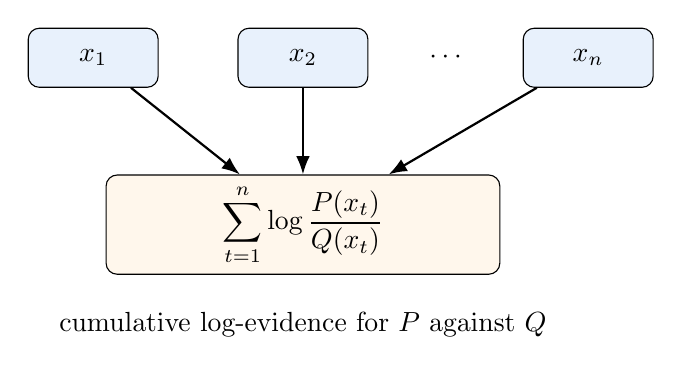
\begin{tikzpicture}[>=Latex,node distance=1.0cm]
\node[draw,rounded corners,fill=lightblue,minimum width=1.65cm,minimum height=0.75cm] (x1) {$x_1$};
\node[draw,rounded corners,fill=lightblue,minimum width=1.65cm,minimum height=0.75cm,right=of x1] (x2) {$x_2$};
\node[right=0.65cm of x2] (dots) {$\cdots$};
\node[draw,rounded corners,fill=lightblue,minimum width=1.65cm,minimum height=0.75cm,right=0.65cm of dots] (xn) {$x_n$};
\node[draw,rounded corners,fill=lightorange,minimum width=5.0cm,minimum height=0.85cm,below=1.1cm of x2] (sum) {$\displaystyle \sum_{t=1}^{n}\log\frac{P(x_t)}{Q(x_t)}$};
\draw[->,thick] (x1) -- (sum);
\draw[->,thick] (x2) -- (sum);
\draw[->,thick] (xn) -- (sum);
\node[below=0.35cm of sum] {cumulative log-evidence for $P$ against $Q$};
\end{tikzpicture}
\end{center}

This is why log-likelihood ratios appear everywhere in statistics, information theory, and sequential learning. They are the natural currency in which independent pieces of evidence add.

\section{The sign has a plain meaning}

Let
\[
L_n
=
\log\frac{P(X_1,\ldots,X_n)}{Q(X_1,\ldots,X_n)}.
\]
Then
\[
L_n>0
\quad\Longleftrightarrow\quad
P(X_1,\ldots,X_n)>Q(X_1,\ldots,X_n),
\]
so the observed sample is more likely under $P$.

Similarly,
\[
L_n<0
\quad\Longleftrightarrow\quad
P(X_1,\ldots,X_n)<Q(X_1,\ldots,X_n),
\]
so the observed sample is more likely under $Q$.

The number $L_n$ is random because the data are random. The next question is therefore not whether one particular path rises or falls. It is whether the path has a systematic drift.

\chapter{KL Divergence Is Average Log-Evidence}

Suppose $P$ is the true data-generating distribution. The one-step log-evidence is
\[
\log\frac{P(X)}{Q(X)}.
\]
Its average under the true world $P$ is
\[
\E_{X\sim P}\left[\log\frac{P(X)}{Q(X)}\right].
\]
This is the Kullback--Leibler divergence:
\[
\boxed{
\KL(P\Vert Q)
=
\E_{X\sim P}\left[\log\frac{P(X)}{Q(X)}\right].
}
\]
For a discrete sample space,
\[
\KL(P\Vert Q)
=
\sum_x P(x)\log\frac{P(x)}{Q(x)}.
\]
For densities $p$ and $q$,
\[
\KL(P\Vert Q)
=
\int p(x)\log\frac{p(x)}{q(x)}\,\dd x.
\]

The notation $P\Vert Q$ is deliberately directional. The expectation is taken under $P$. We are asking:

\begin{center}
\emph{If $P$ is true, how much log-evidence does one observation provide against $Q$, on average?}
\end{center}

This interpretation, emphasized in classic information-theoretic treatments such as MacKay's Cambridge lectures and text, is often more useful than calling KL a ``distance'' \cite{mackay2003information,kullback1951information}.

\begin{keyidea}
KL divergence is an evidence rate. If $\KL(P\Vert Q)=0.03$, then one observation contributes about $0.03$ nats of evidence for $P$ against $Q$ on average. Roughly $n\KL(P\Vert Q)$ nats accumulate after $n$ independent observations.
\end{keyidea}

\section{Nats and bits}

Using the natural logarithm gives units called \emph{nats}. Using $\log_2$ gives bits:
\[
\log_2 z
=
\frac{\log z}{\log 2}.
\]
Therefore,
\[
\KL_{\mathrm{bits}}(P\Vert Q)
=
\frac{\KL_{\mathrm{nats}}(P\Vert Q)}{\log 2}.
\]
The mathematics is unchanged. Only the unit changes.

\section{A first numerical reading}

For $P=\Ber(0.62)$ and $Q=\Ber(0.50)$,
\begin{align*}
\KL(P\Vert Q)
&=
0.62\log\frac{0.62}{0.50}
+
0.38\log\frac{0.38}{0.50}\\
&\approx
0.02908.
\end{align*}
After $220$ independent observations, the expected cumulative evidence is
\[
220\times0.02908
\approx
6.40\text{ nats}.
\]
Equivalently, the expected likelihood ratio is not $e^{6.40}$ because expectation and exponentiation do not commute. What $6.40$ means is that the \emph{expected log} likelihood ratio is $6.40$.

That distinction matters. Evidence paths are noisy.

\begin{figure}[H]
\centering

\includegraphics[width=0.93\textwidth]{assets/kl-divergence/evidence_accumulation.pdf}
\caption{Fourteen independent evidence paths generated under $P=\Ber(0.62)$ and compared with $Q=\Ber(0.50)$. Individual paths wander, while their expected slope is $\KL(P\Vert Q)$.}
\end{figure}

\chapter{Bernoulli KL, Derived from the Data}

The Bernoulli case is the smallest model in which all the ideas are visible.

Let
\[
X_t\in\{0,1\},
\qquad
X_t\overset{\mathrm{iid}}{\sim}\Ber(p).
\]
We compare two candidate means $p$ and $q$.

\section{The likelihood of a binary sample}

Let
\[
S_n=\sum_{t=1}^{n}X_t
\]
be the number of successes. Then the number of failures is $n-S_n$.

Under mean $p$,
\[
P_p(X_1=x_1,\ldots,X_n=x_n)
=
\prod_{t=1}^{n}p^{x_t}(1-p)^{1-x_t}.
\]
Collect the powers:
\begin{align*}
\prod_{t=1}^{n}p^{x_t}(1-p)^{1-x_t}
&=
p^{\sum_{t=1}^{n}x_t}
(1-p)^{\sum_{t=1}^{n}(1-x_t)}\\
&=
p^{S_n}(1-p)^{n-S_n}.
\end{align*}
Under mean $q$,
\[
P_q(X_1=x_1,\ldots,X_n=x_n)
=
q^{S_n}(1-q)^{n-S_n}.
\]

\section{The sample log-likelihood ratio}

Divide the two likelihoods:
\begin{align*}
\frac{P_p(X_{1:n})}{P_q(X_{1:n})}
&=
\frac{p^{S_n}(1-p)^{n-S_n}}
{q^{S_n}(1-q)^{n-S_n}}\\
&=
\left(\frac{p}{q}\right)^{S_n}
\left(\frac{1-p}{1-q}\right)^{n-S_n}.
\end{align*}
Take logs:
\begin{align*}
L_n(p,q)
&=
\log\frac{P_p(X_{1:n})}{P_q(X_{1:n})}\\
&=
S_n\log\frac{p}{q}
+
(n-S_n)\log\frac{1-p}{1-q}.
\end{align*}
Write $\widehat p_n=S_n/n$:
\begin{align*}
L_n(p,q)
&=
n\widehat p_n\log\frac{p}{q}
+n(1-\widehat p_n)\log\frac{1-p}{1-q}\\
&=
n\left[
\widehat p_n\log\frac{p}{q}
+(1-\widehat p_n)\log\frac{1-p}{1-q}
\right].
\end{align*}

\section{Take the expectation under the true mean}

Because $\E_p[\widehat p_n]=p$,
\begin{align*}
\E_p[L_n(p,q)]
&=
n\left[
\E_p[\widehat p_n]\log\frac{p}{q}
+
\E_p[1-\widehat p_n]\log\frac{1-p}{1-q}
\right]\\
&=
n\left[
p\log\frac{p}{q}
+
(1-p)\log\frac{1-p}{1-q}
\right].
\end{align*}
Define
\[
\boxed{
\kl(p,q)
=
p\log\frac{p}{q}
+(1-p)\log\frac{1-p}{1-q}.
}
\]
Then
\[
\boxed{
\E_p[L_n(p,q)]
=
n\,\kl(p,q).
}
\]

The formula is not an arbitrary definition placed on top of the problem. It is what remains after we average the log-likelihood ratio generated by the observations.

\begin{resultbox}
For Bernoulli observations, $\kl(p,q)$ is the expected one-sample log-evidence for mean $p$ against mean $q$.
\end{resultbox}

\chapter{Why KL Is Never Negative}

A single observation can favor the wrong model. A run of observations can also favor the wrong model. KL says that when $P$ is true, the average log-evidence cannot systematically favor $Q$.

The proof uses one elementary inequality:
\[
\log u\le u-1,
\qquad u>0.
\]
Equivalently,
\[
-\log u\ge 1-u.
\]
Set
\[
u(x)=\frac{Q(x)}{P(x)}.
\]
Then
\begin{align*}
\KL(P\Vert Q)
&=
\sum_xP(x)\log\frac{P(x)}{Q(x)}\\
&=
\sum_xP(x)\left[-\log\frac{Q(x)}{P(x)}\right]\\
&\ge
\sum_xP(x)\left[1-\frac{Q(x)}{P(x)}\right]\\
&=
\sum_xP(x)-\sum_xQ(x)\\
&=
1-1\\
&=
0.
\end{align*}
Hence
\[
\boxed{\KL(P\Vert Q)\ge0.}
\]

The inequality $-\log u\ge1-u$ becomes equality only at $u=1$. Therefore, under the usual absolute-continuity conditions,
\[
\KL(P\Vert Q)=0
\quad\Longleftrightarrow\quad
P=Q
\quad\text{almost surely.}
\]

\begin{thinkbox}
Nonnegative does not mean every observation helps. It means helpful observations win on average when the data truly come from $P$.
\end{thinkbox}

\section{Why it is not an ordinary distance}

An ordinary distance satisfies symmetry:
\[
d(P,Q)=d(Q,P).
\]
KL generally does not:
\[
\KL(P\Vert Q)\ne\KL(Q\Vert P).
\]
There is a simple reason. The first quantity averages under $P$; the second averages under $Q$.

For Bernoulli means,
\[
\kl(0.10,0.05)
\approx0.02065,
\]
while
\[
\kl(0.05,0.10)
\approx0.01671.
\]
The two questions are different:

\begin{itemize}
\item If $0.10$ is true, how surprising is a model that says $0.05$?
\item If $0.05$ is true, how surprising is a model that says $0.10$?
\end{itemize}

The rare-event structure is different in the two worlds, so the evidence rate is different.

\begin{figure}[H]
\centering

\includegraphics[width=0.93\textwidth]{assets/kl-divergence/bernoulli_kl_geometry.pdf}
\caption{For a fixed true mean $p$, the curve $q\mapsto\kl(p,q)$ is minimized at $q=p$. The geometry changes near the boundaries $0$ and $1$.}
\end{figure}

\chapter{The Local Shape: KL Becomes a Quadratic}

KL is not a Euclidean distance globally. Near the truth, however, it looks quadratic.

Fix $p\in(0,1)$ and write
\[
q=p+h,
\]
where $h$ is small. Consider
\[
f(q)=\kl(p,q).
\]
Differentiate with respect to $q$:
\begin{align*}
f'(q)
&=
-\frac{p}{q}
+
\frac{1-p}{1-q}.
\end{align*}
At $q=p$,
\begin{align*}
f'(p)
&=
-\frac{p}{p}
+
\frac{1-p}{1-p}\\
&=
-1+1\\
&=
0.
\end{align*}
Differentiate again:
\begin{align*}
f''(q)
&=
\frac{p}{q^2}
+
\frac{1-p}{(1-q)^2}.
\end{align*}
At $q=p$,
\begin{align*}
f''(p)
&=
\frac{p}{p^2}
+
\frac{1-p}{(1-p)^2}\\
&=
\frac{1}{p}
+
\frac{1}{1-p}\\
&=
\frac{1}{p(1-p)}.
\end{align*}
Taylor's formula gives
\begin{align*}
\kl(p,p+h)
&=
f(p)+f'(p)h+\frac12f''(p)h^2+O(h^3)\\
&=
0+0+\frac{h^2}{2p(1-p)}+O(h^3).
\end{align*}
Therefore,
\[
\boxed{
\kl(p,p+h)
=
\frac{h^2}{2p(1-p)}+O(h^3).
}
\]

The denominator $p(1-p)$ is the Bernoulli variance. The same mean error $h$ is more informative when the observation noise is smaller.

At $p=0.50$,
\[
p(1-p)=0.25.
\]
At $p=0.05$,
\[
p(1-p)=0.0475.
\]
A shift of size $0.02$ is therefore much easier to detect near $0.05$ than near $0.50$.

\section{Fisher information appears automatically}

For the Bernoulli family, the Fisher information in one observation is
\[
I(p)=\frac{1}{p(1-p)}.
\]
The local expansion becomes
\[
\kl(p,p+h)
=
\frac12 I(p)h^2+O(h^3).
\]
This is the precise sense in which KL supplies a local geometry for statistical models. The curvature is not chosen by hand. It is determined by how quickly the likelihood changes.

\begin{researchbox}
This local quadratic structure is the bridge from elementary Bernoulli calculations to exponential families, asymptotic normality, natural gradients, and information geometry. The next chapter will make that bridge explicit.
\end{researchbox}

\section{Hoeffding is the worst-case quadratic shadow}

For Bernoulli means, Pinsker's inequality becomes
\[
\kl(p,q)\ge2(p-q)^2.
\]
A short calculus proof is possible. Fix $q$ and define
\[
g(p)=\kl(p,q)-2(p-q)^2.
\]
Then
\[
g(q)=0.
\]
Also,
\begin{align*}
g'(p)
&=
\log\frac{p(1-q)}{q(1-p)}-4(p-q),\\
g'(q)
&=0.
\end{align*}
Finally,
\begin{align*}
g''(p)
&=
\frac1p+\frac1{1-p}-4\\
&=
\frac{1}{p(1-p)}-4\\
&\ge0,
\end{align*}
where the last step follows from
\[
p(1-p)\le\frac14.
\]
Thus $g$ is convex and has a stationary point at $p=q$. That point is its minimum, so
\[
g(p)\ge g(q)=0.
\]
Hence
\[
\boxed{\kl(p,q)\ge2(p-q)^2.}
\]

This inequality explains the relation between KL-based bounds and Hoeffding bounds. Hoeffding replaces the exact Bernoulli evidence by a universal quadratic lower bound. It is simpler, but it forgets the variance-dependent shape.

\chapter{The Bernoulli Chernoff Bound, Step by Step}

We now derive the tail bound that places KL directly inside confidence intervals and bandit algorithms.

Let
\[
X_1,\ldots,X_n\overset{\mathrm{iid}}{\sim}\Ber(p),
\qquad
\widehat p_n=\frac1n\sum_{t=1}^{n}X_t.
\]
We want an upper bound on
\[
\Pbb_p(\widehat p_n\ge x),
\qquad x>p.
\]

\section{Step 1: turn the event into an exponential event}

For any $\lambda>0$,
\begin{align*}
\widehat p_n\ge x
&\Longleftrightarrow
\sum_{t=1}^{n}X_t\ge nx\\
&\Longleftrightarrow
\exp\left(\lambda\sum_{t=1}^{n}X_t\right)
\ge
\exp(\lambda nx).
\end{align*}

\section{Step 2: apply Markov's inequality}

\begin{align*}
\Pbb_p(\widehat p_n\ge x)
&=
\Pbb_p\left(
\exp\left(\lambda\sum_{t=1}^{n}X_t\right)
\ge e^{\lambda nx}
\right)\\
&\le
\frac{
\E_p\left[
\exp\left(\lambda\sum_{t=1}^{n}X_t\right)
\right]
}{e^{\lambda nx}}.
\end{align*}

\section{Step 3: use independence}

\begin{align*}
\E_p\left[
\exp\left(\lambda\sum_{t=1}^{n}X_t\right)
\right]
&=
\E_p\left[
\prod_{t=1}^{n}e^{\lambda X_t}
\right]\\
&=
\prod_{t=1}^{n}\E_p[e^{\lambda X_t}]\\
&=
\left(\E_p[e^{\lambda X_1}]\right)^n.
\end{align*}
For one Bernoulli variable,
\begin{align*}
\E_p[e^{\lambda X_1}]
&=
(1-p)e^{\lambda\cdot0}+pe^{\lambda\cdot1}\\
&=
1-p+pe^\lambda.
\end{align*}
Therefore,
\[
\Pbb_p(\widehat p_n\ge x)
\le
\exp\left
\{n\left[
\log(1-p+pe^\lambda)-\lambda x
\right]
\right\}.
\]

\section{Step 4: choose the best exponential tilt}

Define
\[
\phi(\lambda)
=
\log(1-p+pe^\lambda)-\lambda x.
\]
Differentiate:
\[
\phi'(\lambda)
=
\frac{pe^\lambda}{1-p+pe^\lambda}-x.
\]
Set $\phi'(\lambda)=0$:
\begin{align*}
\frac{pe^\lambda}{1-p+pe^\lambda}
&=x\\
pe^\lambda
&=x(1-p)+xpe^\lambda\\
pe^\lambda(1-x)
&=x(1-p)\\
e^\lambda
&=
\frac{x(1-p)}{p(1-x)}.
\end{align*}
Thus
\[
\lambda^*
=
\log\frac{x(1-p)}{p(1-x)}.
\]
Because $x>p$, we have $\lambda^*>0$.

\section{Step 5: substitute the optimizer}

First,
\begin{align*}
1-p+pe^{\lambda^*}
&=
1-p+p\frac{x(1-p)}{p(1-x)}\\
&=
1-p+\frac{x(1-p)}{1-x}\\
&=
\frac{(1-p)(1-x)+x(1-p)}{1-x}\\
&=
\frac{1-p}{1-x}.
\end{align*}
Therefore,
\begin{align*}
\phi(\lambda^*)
&=
\log\frac{1-p}{1-x}
-x\log\frac{x(1-p)}{p(1-x)}\\
&=
\log\frac{1-p}{1-x}
-x\log\frac{x}{p}
-x\log\frac{1-p}{1-x}\\
&=
-x\log\frac{x}{p}
+(1-x)\log\frac{1-p}{1-x}\\
&=
-\left[
 x\log\frac{x}{p}
 +(1-x)\log\frac{1-x}{1-p}
\right]\\
&=
-\kl(x,p).
\end{align*}
We have proved
\[
\boxed{
\Pbb_p(\widehat p_n\ge x)
\le
\exp\{-n\kl(x,p)\},
\qquad x>p.
}
\]
Similarly,
\[
\boxed{
\Pbb_p(\widehat p_n\le x)
\le
\exp\{-n\kl(x,p)\},
\qquad x<p.
}
\]

\begin{patternbox}
The proof pattern is:
\[
\text{rare event}
\to
\text{exponential transform}
\to
\text{Markov}
\to
\text{optimize the exponent}
\to
\text{KL divergence}.
\]
This pattern reappears in large deviations, sequential tests, confidence sequences, and bandit analysis.
\end{patternbox}

\section{KL versus Hoeffding}

Pinsker gives
\[
\kl(x,p)\ge2(x-p)^2.
\]
Therefore,
\begin{align*}
\Pbb_p(\widehat p_n\ge x)
&\le
\exp\{-n\kl(x,p)\}\\
&\le
\exp\{-2n(x-p)^2\}.
\end{align*}
The KL-Chernoff bound is at least as sharp as the Hoeffding bound in this Bernoulli setting.

\begin{figure}[H]
\centering

\includegraphics[width=0.93\textwidth]{assets/kl-divergence/tail_bounds_comparison.pdf}
\caption{For $n=100$ and $p=0.20$, the exact binomial upper tail is compared with its KL-Chernoff and Hoeffding upper bounds. KL preserves more of the distribution's shape.}
\end{figure}

\chapter{Confidence Bounds as Inverted Evidence Tests}

A confidence bound asks which candidate means are still plausible after seeing the data.

Suppose the empirical mean is $\widehat p_n$. A candidate upper mean $q\ge\widehat p_n$ becomes harder to believe as
\[
n\kl(\widehat p_n,q)
\]
grows. The quantity has a direct reading:

\begin{center}
\emph{sample size} $\times$ \emph{evidence per sample}.
\end{center}

Given an evidence budget $\beta>0$, define the upper endpoint
\[
U_n
=
\sup\left\{
q\in[\widehat p_n,1]:
 n\kl(\widehat p_n,q)\le\beta
\right\}.
\]
The set
\[
\left\{q:n\kl(\widehat p_n,q)\le\beta\right\}
\]
contains candidate means that the data have not separated strongly enough from the empirical mean.

There is usually no elementary closed form for $U_n$. That is not a practical problem. The left side is increasing in $q$ for $q\ge\widehat p_n$, so binary search finds the endpoint quickly.

\begin{codeblock}{Python}
import numpy as np


def bernoulli_kl(p, q):
    p = np.asarray(p, dtype=float)
    q = np.clip(np.asarray(q, dtype=float), 1e-14, 1 - 1e-14)
    p_safe = np.clip(p, 1e-14, 1 - 1e-14)

    first = p_safe * np.log(p_safe / q)
    second = (1 - p_safe) * np.log((1 - p_safe) / (1 - q))
    first = np.where(p > 0, first, 0.0)
    second = np.where(p < 1, second, 0.0)
    return first + second


def kl_upper_bound(mean, count, beta, steps=28):
    lo = mean.copy()
    hi = np.ones_like(mean)

    for _ in range(steps):
        mid = (lo + hi) / 2
        feasible = count * bernoulli_kl(mean, mid) <= beta
        lo = np.where(feasible, mid, lo)
        hi = np.where(feasible, hi, mid)

    return lo
\end{codeblock}

\section{Why the KL radius changes with the mean}

Using the local approximation
\[
\kl(\widehat p_n,\widehat p_n+h)
\approx
\frac{h^2}{2\widehat p_n(1-\widehat p_n)},
\]
the condition
\[
n\kl(\widehat p_n,\widehat p_n+h)\le\beta
\]
becomes
\begin{align*}
n\frac{h^2}{2\widehat p_n(1-\widehat p_n)}
&\lesssim\beta\\
h^2
&\lesssim
\frac{2\widehat p_n(1-\widehat p_n)\beta}{n}\\
h
&\lesssim
\sqrt{
\frac{2\widehat p_n(1-\widehat p_n)\beta}{n}
}.
\end{align*}
The radius shrinks near $0$ and $1$ because Bernoulli variance shrinks there.

Hoeffding uses the worst-case variance $1/4$ for every mean. It therefore produces an essentially constant radius before clipping at the boundary.

\begin{figure}[H]
\centering

\includegraphics[width=0.93\textwidth]{assets/kl-divergence/confidence_radii.pdf}
\caption{KL and Hoeffding upper radii with the same evidence budget. KL automatically adapts to the Bernoulli variance.}
\end{figure}

\chapter{KL-UCB: Optimism Measured in Evidence}

UCB chooses the action with the largest plausible mean. The simplest version builds plausibility from a quadratic Hoeffding radius:
\[
\widehat\mu_a(t)
+
\sqrt{\frac{2\log t}{N_a(t)}}.
\]
KL-UCB keeps the same optimistic principle but replaces the generic radius by a distribution-aware evidence constraint \cite{garivier2011klucb}.

For Bernoulli rewards, define
\[
U_a(t)
=
\sup\left\{
q\in[\widehat\mu_a(t),1]:
N_a(t)\kl(\widehat\mu_a(t),q)
\le
f(t)
\right\},
\]
where a common exploration function is
\[
f(t)=\log t+c\log\log t.
\]
Then choose
\[
A_t\in\argmax_a U_a(t).
\]

\begin{keyidea}
UCB1 asks how far a mean could move under a universal quadratic error bar. KL-UCB asks which larger means remain statistically difficult to distinguish from the observed arm.
\end{keyidea}

\section{The complete decision rule}

\begin{enumerate}
\item Pull every arm once.
\item For each arm, compute its empirical mean and pull count.
\item Find the largest candidate mean whose KL evidence against the empirical mean is below the exploration budget.
\item Pull the arm with the largest candidate mean.
\item Update only the selected arm.
\end{enumerate}

\begin{codeblock}{Python}
for t in range(number_of_arms, horizon):
    empirical = successes / counts

    log_t = np.log(t + 1.0)
    beta = log_t + 3.0 * np.log(max(log_t, 1.0))

    index = kl_upper_bound(empirical, counts, beta)
    chosen = np.argmax(index, axis=1)

    reward = rng.random(number_of_runs) < true_means[chosen]
    successes[row, chosen] += reward
    counts[row, chosen] += 1
\end{codeblock}

\section{What the asymptotic denominator means}

For a suboptimal Bernoulli arm $a$ with mean $\mu_a<\mu_*$, the classical logarithmic scale is
\[
\E[N_a(T)]
\approx
\frac{\log T}{\kl(\mu_a,\mu_*)}.
\]
The denominator is the evidence obtained from one pull of arm $a$ when we compare its true distribution with an alternative in which it could look as good as the best arm.

Large KL:
\[
\text{one pull is informative}
\quad\Longrightarrow\quad
\text{few pulls are needed}.
\]
Small KL:
\[
\text{the worlds are hard to distinguish}
\quad\Longrightarrow\quad
\text{many pulls are unavoidable}.
\]
This is the deeper meaning of the Lai--Robbins lower bound and the matching behavior of KL-UCB \cite{lai1985,garivier2011klucb,lattimore2020bandit}.

\chapter{Information Adds Across Observations}

Suppose
\[
X_1,\ldots,X_n\overset{\mathrm{iid}}{\sim}P
\]
under one world and
\[
X_1,\ldots,X_n\overset{\mathrm{iid}}{\sim}Q
\]
under another. The joint laws are $P^n$ and $Q^n$.

The likelihood ratio factorizes:
\[
\frac{P^n(X_{1:n})}{Q^n(X_{1:n})}
=
\prod_{t=1}^{n}\frac{P(X_t)}{Q(X_t)}.
\]
Hence
\begin{align*}
\KL(P^n\Vert Q^n)
&=
\E_{P^n}\left[
\log\frac{P^n(X_{1:n})}{Q^n(X_{1:n})}
\right]\\
&=
\E_{P^n}\left[
\sum_{t=1}^{n}\log\frac{P(X_t)}{Q(X_t)}
\right]\\
&=
\sum_{t=1}^{n}
\E_P\left[
\log\frac{P(X_t)}{Q(X_t)}
\right]\\
&=
n\KL(P\Vert Q).
\end{align*}
Thus
\[
\boxed{\KL(P^n\Vert Q^n)=n\KL(P\Vert Q).}
\]

This exact additivity is one reason KL is so central. It turns sample size into an information budget.

\chapter{Information Accounting in an Adaptive Bandit}

The data in a bandit are not iid as a single sequence. The selected arm changes with the history. Nevertheless, KL still adds cleanly.

Consider two bandit environments:
\[
\nu=(P_1,\ldots,P_K),
\qquad
\nu'=(Q_1,\ldots,Q_K).
\]
Use the same algorithm in both environments. Let the history through time $T$ be
\[
H_T=(A_1,X_1,\ldots,A_T,X_T).
\]
The algorithm chooses $A_t$ according to a policy
\[
\pi_t(a\mid H_{t-1}).
\]
Under environment $\nu$, the history density is
\[
p_\nu(H_T)
=
\prod_{t=1}^{T}
\pi_t(A_t\mid H_{t-1})
\,p_{A_t}(X_t).
\]
Under environment $\nu'$, it is
\[
p_{\nu'}(H_T)
=
\prod_{t=1}^{T}
\pi_t(A_t\mid H_{t-1})
\,q_{A_t}(X_t).
\]
Divide:
\begin{align*}
\frac{p_\nu(H_T)}{p_{\nu'}(H_T)}
&=
\frac{
\prod_{t=1}^{T}
\pi_t(A_t\mid H_{t-1})p_{A_t}(X_t)
}{
\prod_{t=1}^{T}
\pi_t(A_t\mid H_{t-1})q_{A_t}(X_t)
}\\
&=
\prod_{t=1}^{T}
\frac{p_{A_t}(X_t)}{q_{A_t}(X_t)}.
\end{align*}
The policy terms cancel. The algorithm reacts differently because its observed histories differ, but conditional on a given history it uses the same rule in both worlds.

Take logs and expectations under $\nu$:
\begin{align*}
\KL(\Pbb_\nu^{H_T}\Vert\Pbb_{\nu'}^{H_T})
&=
\E_\nu\left[
\sum_{t=1}^{T}
\log\frac{p_{A_t}(X_t)}{q_{A_t}(X_t)}
\right]\\
&=
\sum_{t=1}^{T}
\E_\nu\left[
\E_\nu\left[
\left.
\log\frac{p_{A_t}(X_t)}{q_{A_t}(X_t)}
\right|
H_{t-1},A_t
\right]
\right]\\
&=
\sum_{t=1}^{T}
\E_\nu\left[
\KL(P_{A_t}\Vert Q_{A_t})
\right].
\end{align*}
Now use indicators:
\[
\KL(P_{A_t}\Vert Q_{A_t})
=
\sum_{a=1}^{K}
\one\{A_t=a\}\KL(P_a\Vert Q_a).
\]
Therefore,
\begin{align*}
\KL(\Pbb_\nu^{H_T}\Vert\Pbb_{\nu'}^{H_T})
&=
\sum_{t=1}^{T}
\sum_{a=1}^{K}
\E_\nu[\one\{A_t=a\}]
\KL(P_a\Vert Q_a)\\
&=
\sum_{a=1}^{K}
\E_\nu\left[
\sum_{t=1}^{T}\one\{A_t=a\}
\right]
\KL(P_a\Vert Q_a)\\
&=
\boxed{
\sum_{a=1}^{K}
\E_\nu[N_a(T)]
\KL(P_a\Vert Q_a)
}.
\end{align*}

\begin{patternbox}
Bandit information accounting:
\[
\boxed{
\text{total information}
=
\sum_a
\text{expected number of pulls of arm }a
\times
\text{information per pull}.
}
\]
Adaptivity changes the random pull counts. It does not destroy the accounting identity.
\end{patternbox}

\begin{center}
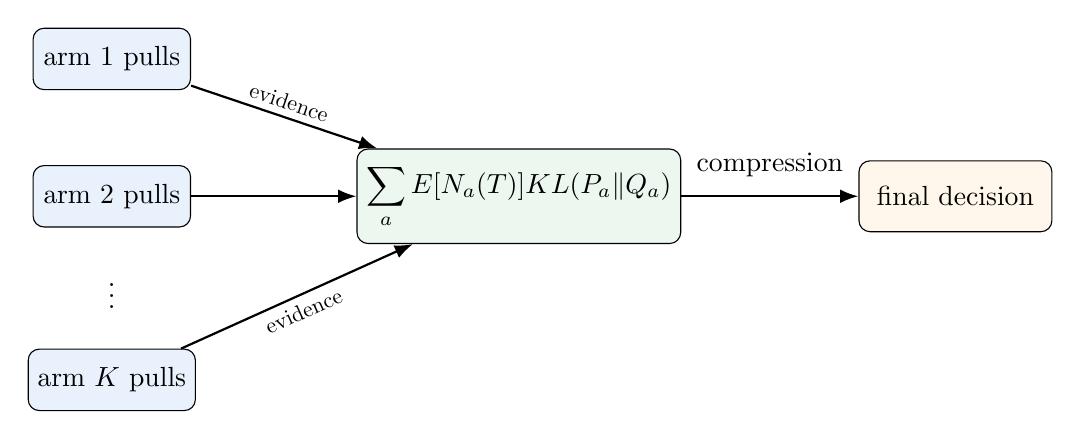
\begin{tikzpicture}[>=Latex,node distance=0.95cm]
\node[draw,rounded corners,fill=lightblue,minimum width=2.0cm,minimum height=0.78cm] (a1) {arm 1 pulls};
\node[draw,rounded corners,fill=lightblue,minimum width=2.0cm,minimum height=0.78cm,below=of a1] (a2) {arm 2 pulls};
\node[below=0.38cm of a2] (dots) {$\vdots$};
\node[draw,rounded corners,fill=lightblue,minimum width=2.0cm,minimum height=0.78cm,below=0.38cm of dots] (ak) {arm $K$ pulls};
\node[draw,rounded corners,fill=softgreen,minimum width=3.25cm,minimum height=1.2cm,right=2.1cm of a2] (budget) {$\displaystyle\sum_a\E[N_a(T)]\KL(P_a\Vert Q_a)$};
\node[draw,rounded corners,fill=lightorange,minimum width=2.45cm,minimum height=0.9cm,right=2.25cm of budget] (decision) {final decision};
\draw[->,thick] (a1) -- node[above,sloped,scale=0.8] {evidence} (budget);
\draw[->,thick] (a2) -- (budget);
\draw[->,thick] (ak) -- node[below,sloped,scale=0.8] {evidence} (budget);
\draw[->,thick] (budget) -- node[midway,above=0.12cm]{compression} (decision);
\end{tikzpicture}
\end{center}

\chapter{A Decision Cannot Contain More Information Than the Data}

An algorithm may observe a long transcript and finally output one bit:
\[
Z=\one\{\text{recommend arm 1}\}.
\]
The output is a compressed version of the history. Compression cannot make two worlds easier to distinguish.

Let $E$ be any event determined by the data. Write
\[
p=P(E),
\qquad
q=Q(E).
\]
The binary KL divergence between the event probabilities is
\[
\kl(p,q)
=
p\log\frac{p}{q}
+(1-p)\log\frac{1-p}{1-q}.
\]
The chain rule for the indicator $Z=\one_E$ gives
\begin{align*}
\KL(P\Vert Q)
&=
\kl(P(E),Q(E))\\
&\quad+
P(E)\KL(P(\cdot\mid E)\Vert Q(\cdot\mid E))\\
&\quad+
P(E^c)\KL(P(\cdot\mid E^c)\Vert Q(\cdot\mid E^c)).
\end{align*}
The last two terms are nonnegative. Therefore,
\[
\boxed{
\KL(P\Vert Q)
\ge
\kl(P(E),Q(E)).
}
\]
This is a binary form of the data-processing inequality.

\begin{keyidea}
The full data may contain subtle evidence. A final yes/no decision can only discard information. Any reliable decision therefore requires enough KL to have accumulated before the compression.
\end{keyidea}

\section{The seed of a lower bound}

Suppose an algorithm must identify the best arm in two nearby environments.

Let
\[
E=\{\text{algorithm outputs arm 1}\}.
\]
In environment $\nu$, arm 1 is best, so a $\delta$-correct algorithm satisfies
\[
\Pbb_\nu(E)\ge1-\delta.
\]
In environment $\nu'$, arm 1 is not best, so
\[
\Pbb_{\nu'}(E)\le\delta.
\]
Data processing gives
\[
\KL(\Pbb_\nu^{H_T}\Vert\Pbb_{\nu'}^{H_T})
\ge
\kl(1-\delta,\delta).
\]
Combine this with bandit information accounting:
\[
\boxed{
\sum_{a=1}^{K}
\E_\nu[N_a(T)]\KL(P_a\Vert Q_a)
\ge
\kl(1-\delta,\delta).
}
\]
For small $\delta$,
\[
\kl(1-\delta,\delta)
\asymp
\log\frac1\delta.
\]
So reliable identification requires a logarithmic amount of evidence.

This is the central research paradigm behind modern bandit lower bounds and best-arm identification \cite{kaufmann2016complexity}. The next chapter will develop the full change-of-measure method carefully.

\chapter{Reproducible Experiment: UCB1, KL-UCB, and Thompson Sampling}

We now run the algorithms in the same four-arm Bernoulli environment:
\[
(\mu_1,\mu_2,\mu_3,\mu_4)
=
(0.03,0.05,0.08,0.12).
\]
The horizon is
\[
T=12000,
\]
and every curve is averaged over $220$ independent runs.

The environment is deliberately near the lower boundary. Bernoulli variance is small there, so a worst-case Hoeffding radius wastes substantial information.

\section{Pseudo-regret}

Let
\[
\mu_*=0.12.
\]
The cumulative pseudo-regret is
\[
R_T
=
\sum_{t=1}^{T}(\mu_*-\mu_{A_t}).
\]
It depends on the selected arms, not on the realized reward noise. This makes the comparison easier to read.

\begin{figure}[H]
\centering

\includegraphics[width=0.94\textwidth]{assets/kl-divergence/kl_ucb_regret.pdf}
\caption{Mean cumulative pseudo-regret. KL-UCB uses the Bernoulli evidence geometry and avoids much of the over-exploration of UCB1. Thompson sampling is included as a posterior-sampling reference.}
\end{figure}

\section{Where the samples went}

\begin{figure}[H]
\centering

\includegraphics[width=0.94\textwidth]{assets/kl-divergence/kl_ucb_pull_counts.pdf}
\caption{Mean pull counts after $12000$ rounds. Better evidence accounting means fewer pulls of clearly inferior arms.}
\end{figure}

\begin{table}[H]
\centering
\caption{Simulation summary. Values are means over $220$ runs.}
\begin{tabular}{lrrrrr}
\toprule
Algorithm & Regret & Arm 1 & Arm 2 & Arm 3 & Arm 4 \\
\midrule
UCB1 & 270.64 & 967.43 & 1303.31 & 2308.53 & 7420.74 \\
KL-UCB & 86.20 & 227.61 & 372.99 & 990.07 & 10409.33 \\
Thompson sampling & 37.42 & 103.01 & 156.88 & 429.17 & 11310.94 \\
\bottomrule
\end{tabular}
\end{table}

The experiment is not a theorem. Different instances and horizons can change the numerical ranking. The durable lesson is structural:

\[
\text{a confidence rule that matches the reward model}
\]
can use observations more efficiently than
\[
\text{a confidence rule built from a worst-case surrogate}.
\]

\chapter{Three Ways KL Reappears in Machine Learning}

\section{Variational inference: approximation by information loss}

Suppose $p(z\mid x)$ is a difficult posterior and $q(z)$ is a tractable approximation. Variational inference often minimizes
\[
\KL(q(z)\Vert p(z\mid x)).
\]
The same divergence now measures the average log mismatch when samples come from the approximation $q$. The direction matters: reversing the arguments changes which parts of the posterior are expensive to miss.

This probabilistic-learning view is part of the Cambridge tradition associated with MacKay and Ghahramani: probability models are not decorative wrappers around algorithms; they determine the objective and the geometry \cite{mackay2003information,ghahramani2015probabilistic}.

\section{Information gain: expected posterior movement}

Mutual information is an expected KL divergence:
\[
I(\Theta;Y)
=
\E_Y\left[
\KL\bigl(P(\Theta\mid Y)\Vert P(\Theta)\bigr)
\right].
\]
It measures how far the posterior is expected to move after seeing $Y$.

This idea drives information-directed sampling and information-based Bayesian optimization. In work connected to ETH Zurich, information gain controls regret in Gaussian-process and heteroscedastic bandits \cite{srinivas2010gpucb,kirschner2018information}. Oxford work on information-theoretic Bayesian optimization similarly chooses evaluations for their expected reduction of uncertainty about the optimum \cite{ru2018fast}.

\section{Bandit lower bounds and best-arm identification}

In best-arm identification, the learner must collect enough evidence to rule out every alternative world in which another arm is best. Each arm contributes evidence at a rate determined by KL. The sample allocation problem is therefore an information allocation problem.

This viewpoint is central to the lower bounds and algorithms of Kaufmann, Cappe, and Garivier \cite{kaufmann2016complexity}, and it continues in recent work on minimal-regret best-arm identification by Yang, Tan, and Tianyuan Jin \cite{yang2024minimal}. Their Double KL-UCB construction makes the connection especially explicit: confidence bounds are not only a technical device; they are the mechanism by which regret and identification evidence are jointly managed.

\chapter{Common Misreadings}

\section{``KL is the distance between two parameter values''}

Not exactly. KL compares probability laws. Parameters enter only through the distributions they define.

For Bernoulli models,
\[
p\mapsto\Ber(p),
\]
so writing $\kl(p,q)$ is harmless shorthand. In a different model family, the same numerical parameter gap may generate a very different KL divergence.

\section{``Large KL means the models are far apart in every sense''}

KL is tailored to statistical discrimination. It need not agree with Euclidean distance, Wasserstein distance, or total variation. Different divergences answer different questions.

\section{``KL is symmetric enough when the parameters are close''}

Locally, both directions share the same leading quadratic term:
\[
\KL(P_\theta\Vert P_{\theta+h})
=
\frac12h^\top I(\theta)h+o(\|h\|^2).
\]
But outside a small neighborhood, direction can matter greatly.

\section{``A KL confidence set is automatically valid at every time''}

No. The shape of a confidence set and its time validity are separate issues. The martingale chapter explained why repeated monitoring requires time-uniform control. A KL-shaped boundary can be fixed-time or anytime-valid depending on how the threshold is calibrated.

\chapter{What to Carry Forward}

A likelihood ratio compares how well two worlds explain the same observation.

A log-likelihood ratio makes evidence additive.

KL divergence is the expected log-likelihood ratio under the true world.

For Bernoulli observations,
\[
\kl(p,q)
=
p\log\frac pq+(1-p)\log\frac{1-p}{1-q}.
\]
Near the truth,
\[
\kl(p,p+h)
\approx
\frac{h^2}{2p(1-p)}.
\]
For independent observations,
\[
\KL(P^n\Vert Q^n)=n\KL(P\Vert Q).
\]
For an adaptive bandit,
\[
\KL(\Pbb_\nu^{H_T}\Vert\Pbb_{\nu'}^{H_T})
=
\sum_a\E_\nu[N_a(T)]\KL(P_a\Vert Q_a).
\]
For any final decision event $E$,
\[
\KL(P\Vert Q)
\ge
\kl(P(E),Q(E)).
\]
Together, these identities say:
\[
\boxed{
\text{samples create evidence,}
\quad
\text{actions allocate evidence,}
\quad
\text{decisions consume evidence.}
}
\]
That is the role of KL divergence in bandit theory.

\backmatter
\chapter*{Appendix A. Formula Sheet}
\addcontentsline{toc}{chapter}{Appendix A. Formula Sheet}

\begin{table}[H]
\centering
\caption*{Core formulas.}
\begin{tabular}{p{0.34\textwidth}p{0.56\textwidth}}
\toprule
Object & Formula \\
\midrule
Likelihood ratio & $P(x)/Q(x)$ \\
Log-likelihood ratio & $\log(P(x)/Q(x))$ \\
KL divergence & $\KL(P\Vert Q)=\E_P[\log(P(X)/Q(X))]$ \\
Bernoulli KL & $\kl(p,q)=p\log(p/q)+(1-p)\log((1-p)/(1-q))$ \\
Nonnegativity & $\KL(P\Vert Q)\ge0$ \\
Local Bernoulli expansion & $\kl(p,p+h)=h^2/[2p(1-p)]+O(h^3)$ \\
Bernoulli Pinsker & $\kl(p,q)\ge2(p-q)^2$ \\
KL-Chernoff upper tail & $\Pbb_p(\widehat p_n\ge x)\le e^{-n\kl(x,p)}$, $x>p$ \\
KL upper endpoint & $\sup\{q\ge\widehat p:n\kl(\widehat p,q)\le\beta\}$ \\
Product additivity & $\KL(P^n\Vert Q^n)=n\KL(P\Vert Q)$ \\
Bandit information identity & $\KL(\Pbb_\nu^{H_T}\Vert\Pbb_{\nu'}^{H_T})=\sum_a\E_\nu[N_a(T)]\KL(P_a\Vert Q_a)$ \\
Binary data processing & $\KL(P\Vert Q)\ge\kl(P(E),Q(E))$ \\
Mutual information & $I(\Theta;Y)=\E_Y[\KL(P(\Theta\mid Y)\Vert P(\Theta))]$ \\
\bottomrule
\end{tabular}
\end{table}

\chapter*{Appendix B. Notation Table}
\addcontentsline{toc}{chapter}{Appendix B. Notation Table}

\begin{table}[H]
\centering
\caption*{Notation.}
\begin{tabular}{p{0.24\textwidth}p{0.66\textwidth}}
\toprule
Symbol & Meaning \\
\midrule
$P,Q$ & competing probability distributions \\
$p,q$ & Bernoulli means or probability mass/density functions, according to context \\
$X_t$ & observation at time $t$ \\
$S_n$ & number of Bernoulli successes in $n$ observations \\
$\widehat p_n$ & empirical Bernoulli mean $S_n/n$ \\
$L_n(P,Q)$ & cumulative log-likelihood ratio for $P$ against $Q$ \\
$\KL(P\Vert Q)$ & expected log-evidence under $P$ against $Q$ \\
$\kl(p,q)$ & binary/Bernoulli KL divergence \\
$A_t$ & arm chosen at time $t$ \\
$N_a(T)$ & number of pulls of arm $a$ through time $T$ \\
$H_T$ & complete bandit history through time $T$ \\
$U_a(t)$ & upper confidence index of arm $a$ \\
$\delta$ & target error probability \\
$\beta$ & evidence threshold used in a confidence set \\
\bottomrule
\end{tabular}
\end{table}

\chapter*{Appendix C. Minimal Implementation Notes}
\addcontentsline{toc}{chapter}{Appendix C. Minimal Implementation Notes}

The supplied Python script produces every figure and table in this note. The two numerically important details are:

\begin{enumerate}
\item Clip candidate probabilities away from exactly $0$ and $1$ before taking logs.
\item Preserve the correct limiting convention $0\log0=0$ when an empirical mean is exactly $0$ or $1$.
\end{enumerate}

The KL-UCB endpoint is monotone and can be found by binary search. Nineteen to thirty iterations are usually more than enough for double-precision simulation.

\chapter*{Further Reading}
\addcontentsline{toc}{chapter}{Further Reading}

MacKay's \emph{Information Theory, Inference, and Learning Algorithms} is an unusually clear route from likelihood ratios to modern probabilistic learning. Lattimore and Szepesvari place KL directly inside the language of bandits. Garivier and Cappe develop KL-UCB. Kaufmann, Cappe, and Garivier show how KL becomes an information budget for best-arm identification. For information-directed algorithms, the work of Russo and Van Roy and the ETH line around Krause provide the natural continuation.


\chapter*{Appendix D. Full Experiment Script}
\addcontentsline{toc}{chapter}{Appendix D. Full Experiment Script}

\lstinputlisting[style=blogcode,language=Python]{assets/kl-divergence/kl_divergence_simulation.py}

\nocite{kullback1951information,mackay2003information,cover2006elements,lattimore2020bandit,lai1985,garivier2011klucb,kaufmann2016complexity,russo2016information,srinivas2010gpucb,kirschner2018information,ru2018fast,ghahramani2015probabilistic,jin2022expts,yang2024minimal}
\printbibliography

\end{document}
